\section{Theorie}
\label{sec:theorie}
Die Bestimmung der diskreten Energiewerte in der Atomhülle kann durch
angelgte Felder und emittierte und absorbierte Strahlung erfolgen,
oder wie im Franck-Hertz-Versuch durch Elektronenstöße.
Auf Grund der Übersichtlichkeit wird Quecksilber mit Hg und Elektron mit
$\symup{e}^{-}$ bezeichnet.

\subsection{Aufbau und Funktionsweise der Franck-Hertz-Apparatur}
Die Apparatur, wie sie in Abbildung \ref{fig:franckaufbau} zusehen ist, besteht
aus einem evakuierten Gefäß in welchems eine kleine Menge an Quecksilber ist.
Gemäß der Dampfdruckkurve in der Versuchsamleitung \cite{Anleitung}
verdampft das Quecksilber und es stellt sich ein Sättigungsdruck ein.
Durch die angelegte Heizspannung kann die Dampfdichte des Gases gesteuert werden.

\begin{figure}
    \centering
    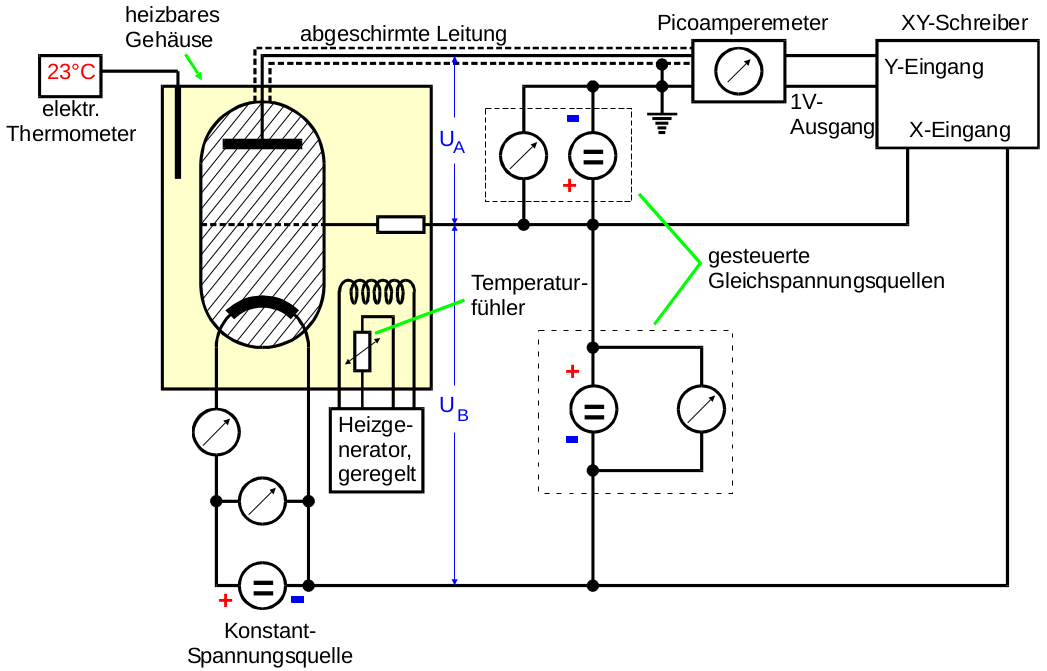
\includegraphics[width=0.7\textwidth]{content/aufbau_franck-hertz.png}
    \caption{Schematischer Aufbau einer Franck-Hertz-Apparatur. \cite{Anleitung}}
    \label{fig:franckaufbau}
\end{figure}

Die $\symup{e}^{-}$ werden aus einem Glühdraht durch den glühelektrischen Effekt
herausgelöst und durch ein elektrisches Feld beschleunigt, sodass für ihre Energie gilt
\begin{equation}
    \frac{\symup{m}_0 v^2}{2} = \symup{e}_0 U_\text{B}\:.
    \label{eqn:beschleunigung}
\end{equation}
Nach der Beschleunigungselektrode werden die $\symup{e}^{-}$ durch ein Gegenfeld abgebremst,
dies ist notwendig zur Energiebestimmung.
Die freie Weglänge zwischen den Hg-Atomen ist für den Versuch eine wichtige
Größe. Diese muss klein gegen die Länge der Röhre sein, damit die $\symup{e}^{-}$
mit den Hg-Atomen in großer Zahl wechselwirken. Es gilt
\begin{equation}
    \bar{w} = \frac{0.0029}{p_\text{sät}} = \frac{0.0029}{\num{5.5e7}}\:\exp\!\left(-\frac{6876}{T}\right)\:,
    \label{eqn:wbar}
\end{equation}
mit $\bar{w}\;\text{in}\;\si{\centi\meter},\;p\;\text{in}\;\si{\milli\bar},
\;\text{und}\;T\;\text{in}\;\si{\kelvin}.$

\subsection{Stoßprozesse}
Ist die Energie der $\symup{e}^{-}$ sehr klein kommt es zu elastischen Stößen mit
den Hg-Atomen. Hierbei gibt das $\symup{e}^{-}$, aufgrund des kleinen
Massenverhältnisses nur den Teil $\increment E$ seiner Energie $E$ ab,
\begin{equation}
    \increment E = \frac{4\symup{m}_0M}{(\symup{m}_0+M)^2}E \approx \num{1.1e-5}E\:.
\end{equation}
Dieses ist der zentrale Stoß, hier ist er wegen seines sehr kleinen
Einflusses zu vernachlässigen.

Interessanter ist der Fall wenn das $\symup{e}^{-}$ auf eine Geschwindigkeit $v$
beschleunigt wurde, sodass die Energie $E$ des $\symup{e}^{-}$ größer gleich des
Energieunterschiedes zwischen dem Grund- und ersten angeregten Zustand des
Hg-Atoms ist,
\begin{align}
    E_{e^{-}} &\geq E_1 - E_0\:.
    \label{eqn:ediff}
    \intertext{Trifft dieses $\symup{e}^{-}$ auf ein Hg-Atom wird dieses angeregt und die
    Energiedifferenz \eqref{eqn:ediff} geht vom $\symup{e}^{-}$ auf das Hg-Atom über,
    dass nach dem Stoß gilt}
    E_{e^{-}}' &= E_{e^{-}} - (E_1 - E_0)\:.
    \intertext{Das Hg-Atom verlässt nach einer Relaxationszeit
    $t_\text{r} \propto \SI{e-8}{\second}$ den angeregten Zustand und kehrt in
    den Grundzustand zurück. Die Energie zwischen den Zuständen wird als Photon mit}
    \symup{h} \nu &= E_1 - E_0
    \label{eqn:gegenfeld}
    \intertext{Die Energie $E_{e^{-}}'$ des $\symup{e}^{-}$ kann nun über ein Gegenfeld
    bestimmt werden, da ein $\symup{e}^{-}$ mit dieser Energie gegen ein elektrisches
    Potential mit der Spannung $U_\text{G}$ nur ankommen kann, wenn gilt}
    E_{e^{-}}' &> \symup{e}_0 U_\text{G}\:.
    \label{eqn:ediffstrich}
\end{align}
abgestrahlt.

\subsection{Franck-Hertz-Kurve}
Die erwartete Form der Kurve $I_\text{A}(U_\text{B})$ hat die in Abbildung
\ref{fig:fhkurve} dargestellte Form. Bei ansteigender Beschleunigungsspannung
steigt der Auffängerstrom $I_\text{A}$ erst an wenn die $\symup{e}^{-}$ das
Gegenfeld überwinden können. Der unstetige Abfall kommt aus der Anregung der
Hg-Atome, da die entsprechende Beschleunigungsspannung die $\symup{e}^{-}$ auf die
benötigte Energie bringt. Diese Form wiederholt sich, wobei die $\symup{e}^{-}$ immer
mehr Atome anregen können.

\begin{figure}
    \centering
    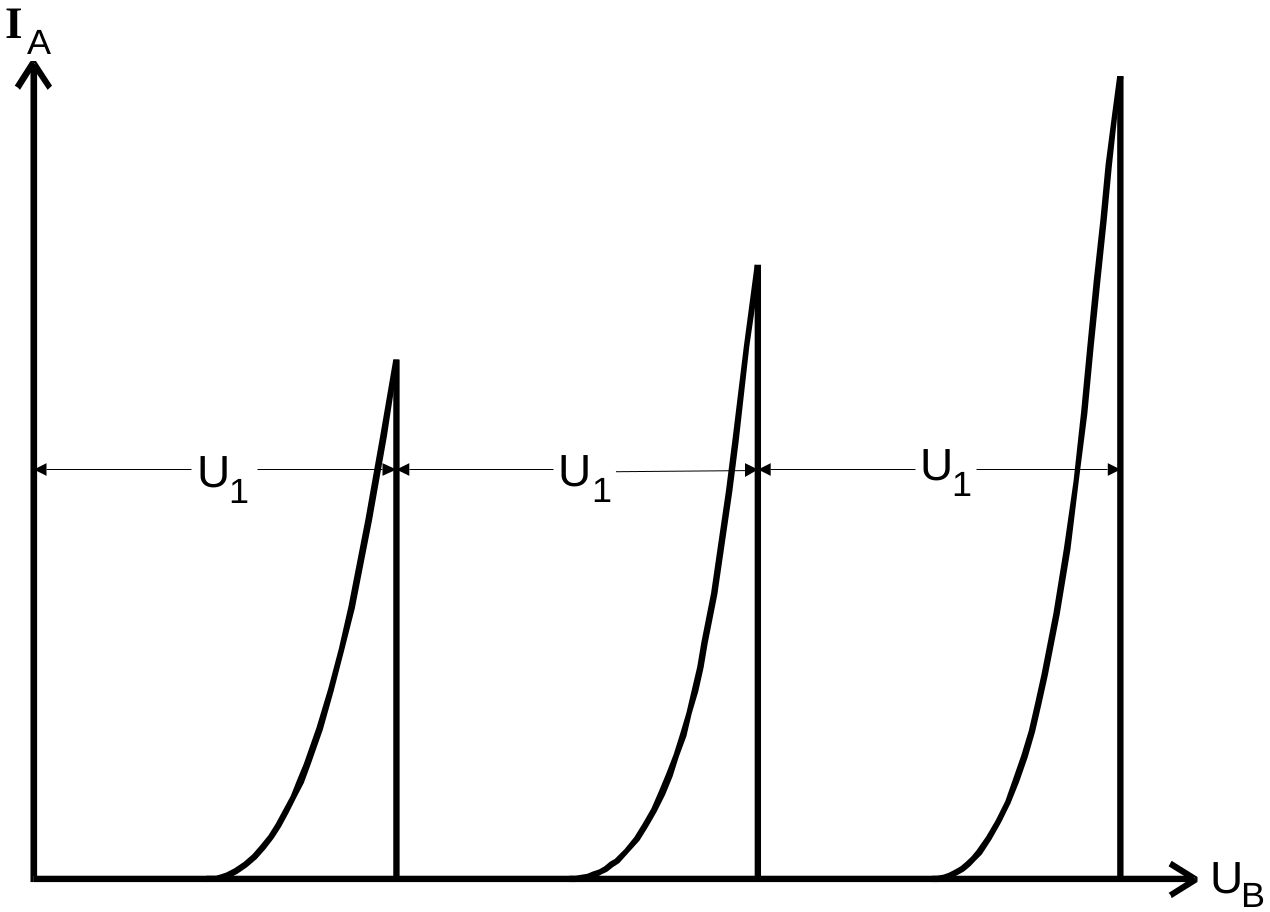
\includegraphics[width=0.65\textwidth]{content/bilder/fhkurve.png}
    \caption{Theoriekurve des Franck-Herrtz-Versuches aus \cite{Anleitung}.}
    \label{fig:fhkurve}
\end{figure}

Die tatsächliche Kurve wird von dieser abweichen, da die $\symup{e}^{-}$ nicht
alle die gleiche Geschwindigkeit in Richtung der Beschleunigung beim Austritt
aus dem Glühdraht haben.
Die Energie der $\symup{e}^{-}$ bei der Emission lässt sich mittels der Fermi-Dirac'schen
Verteilungsfunktion darstellen.
\begin{equation}
  f(\symup{E}) = \frac{1}{\exp \left(\frac{\symup{E}\:-\:ζ}{\symup{kT}}\right)\:+\:1}
\end{equation}
Durch die Verteilung der Energien vor und nach der Beschleunigung
erreicht eine gemessene Kurve ihre Maxima kurz vor der
Theoriekurve und fällt dann stetig gegen die Nulllinie.
Da die Energie der Elektronen kontinuirlich anwächst mit steigender
Beschleunigungsspannung, aber die Anregung nur bei diskreten Energiewerten
geschieht, fällt die Anzahl der an der Anode ankommenden Elektronen
nicht bis auf Null ab.

Jetzt werden noch einmal die elastischen Stöße von oben betrachtet.
Diese führen vor allem im Bereich des Gegenfeldes dazu, dass die
Geschwindigkeitskomponente in Feldrichtung zu klein wird und das $\symup{e}^{-}$
trotz genügend großer Gesamtenergie nicht die Auffangelektrode erreicht.

Ein weiter Effekt der die Kurve verändert ist, dass um den
Wolfram-Glühdraht ein Metall liegt, welches eine geringere Austrittsarbeit hat
um die Ausbeute an $\symup{e}^{-}$ zu maximieren. Die Anode der Beschleunigungsspannung
ist aus einem Material mit hoher Austrittsarbeit, damit die $\symup{e}^{-}$
nicht mit dieser wechselwirken, sondern beschleunigt werden.
Das effektive Beschleunigungspotential zwischen den Elektroden beträgt somit
\begin{equation}
    U_\text{B,eff} = U_\text{B} - \frac{1}{\symup{e}_0} (Φ_\text{B,Ano}- Φ_\text{Glü}) = U_\text{B} - k\:,
    \label{eqn:kontaktpotential}
\end{equation}
mit dem Kontatpotential $k$, um das die Kurve verschoben wird.
